\documentclass{beamer}

\input{../ts-glærur}

\title{FOR3R - Tré, biðraðir, hlaðar og forgangsbiðraðir}

\begin{document}
\begin{frame}
\titlepage
\end{frame}

\section{Inngangur}

\begin{frame}{Upprifjun úr síðasta tíma}
\begin{itemize}
 \item Hnútur (e. \emph{node}) inniheldur gögn og vísun í aðra hnúta
 \item Hægt er að raða hnútum upp í ýmsar gagnagrindur. Við höfum nefnt:
 \begin{itemize}
  \item Eintengda lista
  \item Tvítengda lista
  \item Tré
 \end{itemize}
\end{itemize}
\end{frame}

\section{Tré}

\begin{frame}{Almennt um tré}
\begin{itemize}
 \item Hnútur í tré inniheldur gögn, ásamt vísunum í aðra hnúta
 \item Hnútarnir sem vísað er í eru nefndir börn (e. \emph{children}) hnútarins
 \item Hnútar sem eiga engin börn eru kallaðir lauf (e. \emph{leaves})
 \item Vísanirnar mynda þó aldrei hring!
 \item Í forritun hafa tré oft skilgreindan hámarksfjölda barna, sem trén eru nefnd eftir:
  \begin{itemize}
   \item Að hámarki 2 börn: Tvíundartré (e. \emph{binary tree})
   \item 4 börn: \emph{Quadtree}
   \item 8 börn: \emph{Octree}
  \end{itemize}
\end{itemize}
\end{frame}


\begin{frame}{Hagnýting á tjám: Tvíleitartré}
\begin{itemize}
 \item Sérstök gerð af tvíundartrjám eru svokölluð tvíleitartré (e. \emph{binary search trees})
 \item Tölum um að hver hnútur hafi ``vinstra barn'' og ``hægra barn''
 \item Um tvíleitartré gildir (m.a.):
 \begin{itemize}
  \item Allir vinstri afkomendur hvers hnúts $x$ í trénu hafa lykil sem er \emph{minni} en lykill $x$
  \item Allir hægri afkomendur hvers hnúts $x$ í trénu hafa lykil sem er \emph{stærri} en lykill $x$
  \item Hægt er að ferðast frá ``rót'' trésins að hverjum hnút í trénu
 \end{itemize}
 \item Aths: Hér er ekki gert ráð fyrir endurteknum lyklum
\end{itemize}
\end{frame}

\begin{frame}[fragile]{Leit í tré - sauðakóði}

\begin{verbatim}
tree_search(x,k)
  if x == nil or k == x.key
    return x
  if k < x.key
    return tree_search(x.left,k)
  else
    return tree_search(x.right,k)
\end{verbatim}
Þetta reiknirit hefur sömu eiginleika og helmingunarleit fyrir fylki. (En munið hversu mikið erfiðari sú útfærsla var!)
\end{frame}

\begin{frame}{Hagnýtingarmöguleikar trjáa}
\begin{itemize}
 \item Tré má m.a. nota við
  \item Ýmiss konar leit (oftast tvíleitartré)
  \begin{itemize}
   \item Vísar í gagnasöfnum?
  \end{itemize}
  \item Gervigreind
  \item Framsetning á rými (oft quad- og octrees)
  \begin{itemize}
   \item Tölvuleikir!
  \end{itemize}
\end{itemize}
\end{frame}

\begin{frame}{Ákvarðanir}
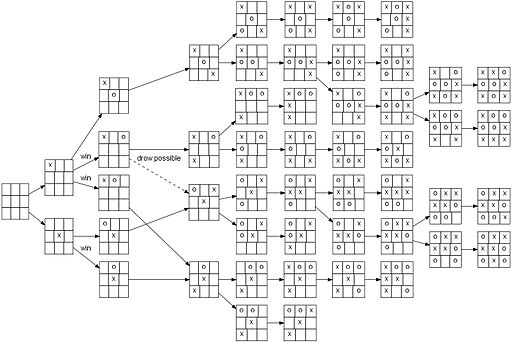
\includegraphics[width=\textwidth]{Pics/tictactoe}
\end{frame}

\begin{frame}{Rýmisskipting}
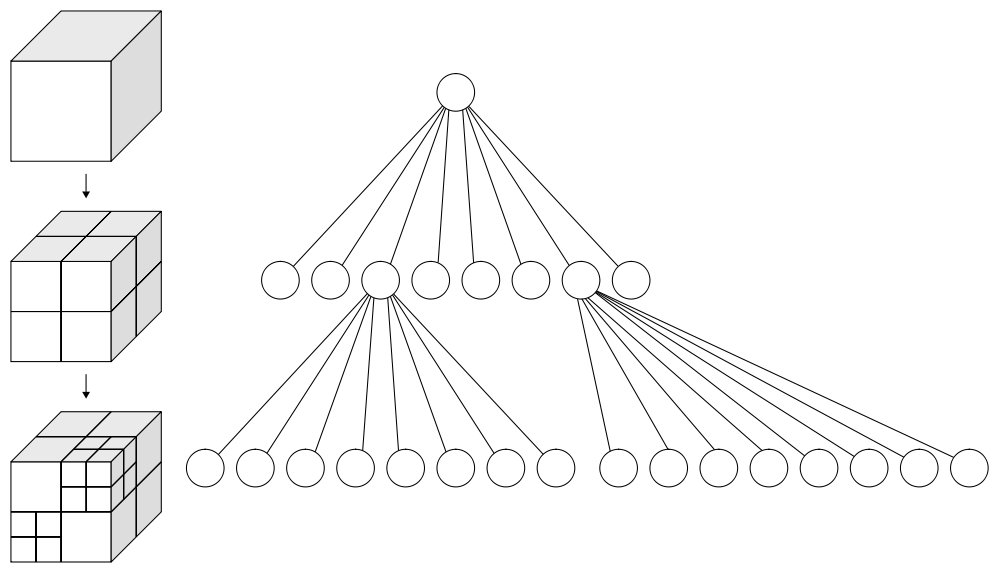
\includegraphics[width=\textwidth]{Pics/octree}
\end{frame}

\begin{frame}{Fleiri góðar gagnagrindur}
\begin{itemize}
 \item Skoðum þrjár
 \begin{itemize}
  \item Biðröð
  \item Hlaði
  \item Forgangsbiðröð
 \end{itemize}
 \item Allar byggjast þær fyrst og fremst á því að geyma gögn og hafa umsjón með því hvernig þau eru tekin út aftur
\end{itemize}
\end{frame}

\section{Biðraðir}

\begin{frame}{Biðraðir}
\begin{columns}[c]
\column{0.5\textwidth}
\begin{itemize}
 \item Biðröð (e. \emph{queue}) er ``First-in, first-out'' (FIFO) gagnagrind
 \item Skilgreinist af tveimur aðferðum:
 \begin{itemize}
  \item \texttt{enqueue} - bætir nýju staki við biðröðina
  \item \texttt{dequeue} - fjarlægir það stak úr biðröðinni sem lengst hefur verið í henni og skilar því
 \end{itemize}
 \item Í útfærslu er biðröð oft byggð ofan á fylki
\end{itemize}
\column{0.5\textwidth}
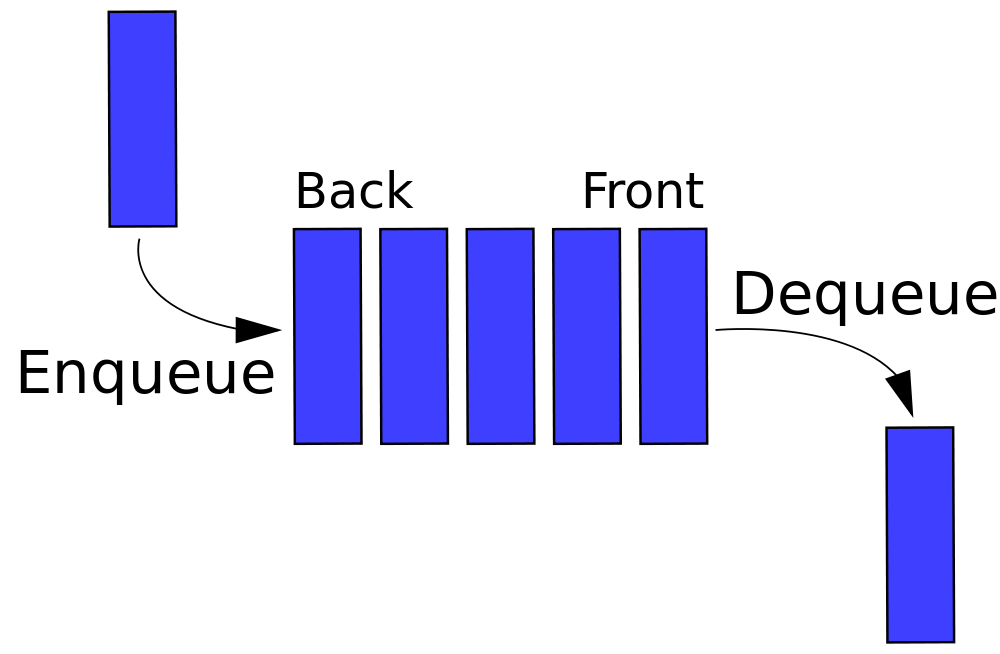
\includegraphics[width=\linewidth]{Pics/queue}
\end{columns}
\end{frame}

\section{Hlaðar}

\begin{frame}{Hlaðar}
\begin{columns}[c]
\column{0.5\textwidth}
\begin{itemize}
 \item Hlaði (e. \emph{stack}) er ``Last-in, first-out'' (LIFO) gagnagrind
 \item Skilgreinist af tveimur aðferðum:
 \begin{itemize}
  \item \texttt{push} - bætir nýju staki á hlaðann
  \item \texttt{pop} - fjarlægir það stak af hlaðanum sem lengst hefur verið á honum og skilar því
  \item Einnig er hægt að skilgreina \texttt{peek} aðferð til að skoða efsta stakið án þess að eyða því af hlaðanum
 \end{itemize}
\end{itemize}
\column{0.5\textwidth}
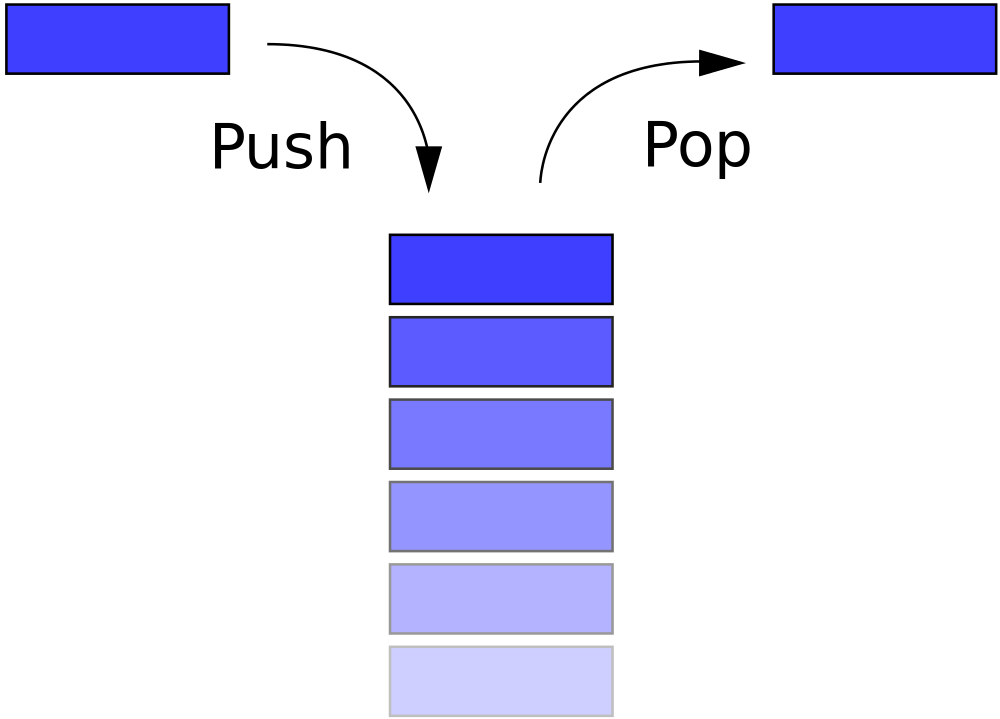
\includegraphics[width=\linewidth]{Pics/stack}
\end{columns}
\end{frame}

\section{Forgangsbiðraðir}

\begin{frame}{Forgangsbiðraðir}
\begin{itemize}
 \item Forgangsbiðröð (e. \emph{priority queue}) skilgreinist af tveimur aðferðum:
 \begin{itemize}
  \item \texttt{insert} - tekur við staki ásamt forgangi og bætir því við forgangsbiðröðina
  \begin{itemize}
   \item Venjulega er ``forgangurinn'' bara tala
  \end{itemize}
  \item \texttt{pull} - fjarlægir það stak úr forgangsbiðröðinni sem hæstan forgang hefur og skilar því
  \item Einnig er \texttt{peek} nær alltaf útfært
 \end{itemize}
 \item Líta má á forgangsbiðröð sem almennari útgáfu af biðröð og/eða hlaða
 \begin{itemize}
  \item Hægt er að nota forgangsbiðröð til að útfæra hinar gagnagrindurnar tvær!
 \end{itemize}
\end{itemize}
\end{frame}


\end{document}
